\documentclass[12 pt]{article}
\usepackage[utf8]{inputenc}
\usepackage[spanish,mexico]{babel}
\usepackage{amsmath}
\usepackage{amssymb}
\usepackage{graphicx}
\usepackage{amsfonts}
\usepackage{float}


\begin{document}
\title{Actividad 9: Aproximación al cálculo del periodo del péndulo}
\author{Luisa Fernanda Orci Fernández}
\date{1 de Mayo de 2016}
\maketitle
\section*{Descripción de la actividad}
Para esta actividad se nos pidió demostrar utilizando Maxima que el periodo del péndulo se puede expresar de la siguiente manera:
	$$T=2\pi \sqrt{\frac{l}{g}}( 1+\frac{1}{16}\theta_{0}^2+\frac{11}{3072}\theta_{0}^4+\frac{173}{737280}\theta_{0}^6+\frac{22931}{1321205760}\theta_{0}^8+\frac{1319183}{951268147200}\theta_{0}^10+...)$$, utilizando como referencia la integral que resolvimos para la actividad anterior, así como también reproducir una gráfica en Python que se asemejara a la propuesta por el artículo de Wikipedia, la cual representa los errores relativos de los periodos.\\
	A continuación se presentan los códigos utilizados para cada una de estas actividades, así como los resultados obtenidos.
	\section*{Procedimiento}
	\subsection*{Demostración de la expresión del periodo}
	Utilizamos Maxima como herramienta para reducir la expresión y seguimos una serie de pasos que a continuación se presentan:
	\begin{itemize}
		\item Comenzamos por definir una función que depende de un parámetro k:
		\begin{verbatim}
		/* Funcion L que depende de un parametro k */
		
		L1(k) := 1/sqrt(1-(k*sin(u))**2);
		\end{verbatim}
		\[\mathrm{L1}\left( k\right) :=\frac{1}{\sqrt{1-{\left( k\,\mathrm{sin}\left( u\right) \right) }^{2}}}\]
		\item Seguimos con una expansión de Taylor...
		\begin{verbatim}
		
		/* Desarrollo por Taylor*/
		
		taylor(1/sqrt(1-k^2*sin(u)^2),u,0,8);
		
		\end{verbatim}
		\[(\%o2)/T/ 1+\frac{{k}^{2}\,{u}^{2}}{2}+\frac{\left( 9\,{k}^{4}-4\,{k}^{2}\right) \,{u}^{4}}{24}+\frac{\left( 225\,{k}^{6}-180\,{k}^{4}+16\,{k}^{2}\right) \,{u}^{6}}{720}\]  \[+\frac{\left( 11025\,{k}^{8}-12600\,{k}^{6}+3024\,{k}^{4}-64\,{k}^{2}\right) \,{u}^{8}}{40320}+...\]
		\item Seguimos desarrollando la expresión a partir de los siguientes pasos que se incluyen:
		\item \begin{verbatim}
		/* Definimos otra funcion L2*/
		
		define(L2(k), %);
		\end{verbatim}
	\[(\%o3)/T/ \mathrm{L2}\left( k\right) :=1+\frac{{k}^{2}\,{u}^{2}}{2}+\frac{\left( 9\,{k}^{4}-4\,{k}^{2}\right) \,{u}^{4}}{24}+\frac{\left( 225\,{k}^{6}-180\,{k}^{4}+16\,{k}^{2}\right) \,{u}^{6}}{720}+\]  \[\frac{\left( 11025\,{k}^{8}-12600\,{k}^{6}+3024\,{k}^{4}-64\,{k}^{2}\right) \,{u}^{8}}{40320}+...\]

	\item \begin{verbatim}
	/* Seno del angulo theta  */
	
	define(x(%theta), sin(%theta));
	\end{verbatim}
\[(\%o13) \mathrm{x}\left( \theta\right) :=\mathrm{sin}\left( \theta\right) \]
\item \begin{verbatim}
/* Integral de L2(k) de cero a 90 grados */

expand(integrate(K2(k),u,0,%pi/2));
\end{verbatim}
\[(\%o14) \frac{\pi \,\mathrm{K2}\left( k\right) }{2}\]
\item \begin{verbatim}/* Sustituimos en la integral anterior el seno de theta */

subst(x(%theta/2), k, %);
\end{verbatim}
\[(\%o15) \frac{\pi \,\mathrm{K2}\left( \mathrm{sin}\left( \frac{\theta}{2}\right) \right) }{2}\]
\item \begin{verbatim}
/* Factorizamos pi/2 */

% *2/%pi;
\end{verbatim}
\[(\%o16) \mathrm{K2}\left( \mathrm{sin}\left( \frac{\theta}{2}\right) \right) \]
\item \begin{verbatim}
/* Definimos ahora una funcion L que depende solo del angulo theta */

define(L(%theta),expand(%));
\end{verbatim}
\[(\%o26) \mathrm{L}\left( \theta\right) :=\mathrm{K2}\left( \mathrm{sin}\left( \frac{\theta}{2}\right) \right) \]

\item \begin{verbatim}
/* Definimos la funcion*/

define(T(%theta),(2*%pi)*sqrt(l/g)*(F(%theta)));
\end{verbatim}
\[(\%o27) \mathrm{T}\left( \theta\right) :=2\,\pi \,\mathrm{K2}\left( \mathrm{sin}\left( \frac{\theta}{2}\right) \right) \,\sqrt{\frac{l}{g}}\]
	\end{itemize}
	Así fue que obtuvimos el desarrollo para llegar a la expresión sugerida.
	
	\subsection*{Gráfica de los errores relativos}
	Para obtener esta gráfica, se utilizó el siguiente código:
	\begin{verbatim}
	import numpy as gatito
import math

#PARAMETROS

g = 9.806
l = 1.00
n = 500
radianesagrad = 180.0/gatito.pi
epsilon = 0.001


#DEFINIMOS ALGUNOS VALORES PARA EL ANGULO INICIAL

theta0 = gatito.linspace(epsilon, gatito.pi-epsilon, n)

#ARREGLOS 

Integral = [0 for i in range(n)]
Integral0 = [0 for i in range(n)]
periodonnum = [0 for i in range(n)]
sine = [0 for i in range(n)]
ere12 = [0 for i in range(n)]

#PERIODO APROXIMADO TEORICO PARA ANGULOS PEQUE;OS

periodot = 2.0*(gatito.pi)*(gatito.sqrt(l/g))

#CALCULAR UN ERROR CON RESPECTO AL TEORICO PARA UNA SERIE DE TERMINOS L

L = 2 
for i in range(0, L):
    for j in range(0,n):
        fac1 = float(math.factorial(2*(i)))
        fac2 = float((2**(i)*math.factorial(i))**2)
        sine[j] = gatito.sin(theta0[j]/2)**(2*(i))
        Integral[j] = ((fac1/fac2)**2)*sine[j]
        Integral0[j] = Integral0[j] + Integral[j]
        periodonnum[j] = 2.0*(gatito.pi)*(gatito.sqrt(l/g)*Integral0[j])
        ere12[j] = periodonnum[j]/periodot
	\end{verbatim}
	Basándonos en una expresión propuesta por el profesor en la página del curso. Al ejecutar dicho código obtuvimos la siguiente gráfica:

\begin{center}
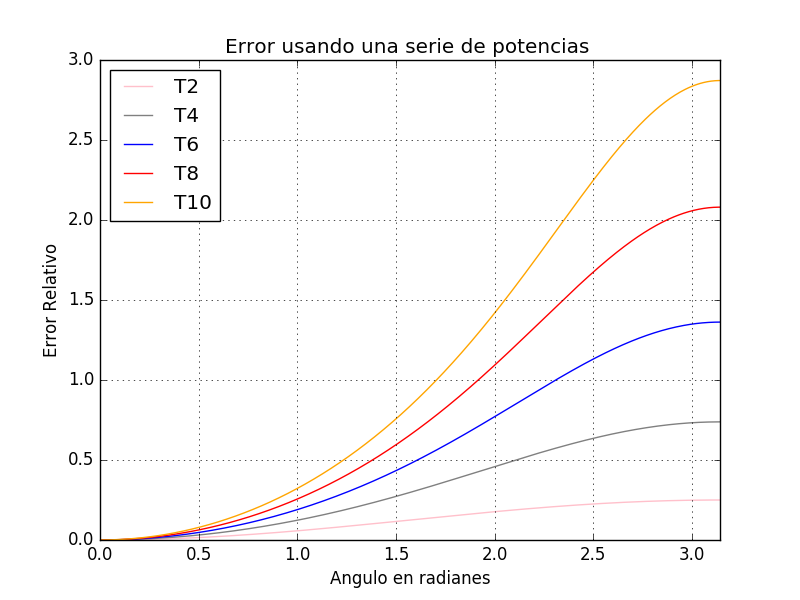
\includegraphics[scale=0.7]{act9.png}
\end{center}	

\section*{Conclusión}
Esta actividad se me hizo dificil al principio por la demostración, pero al momento de poderla terminar, se me fue facilitando poco a poco.


	
\end{document}